\documentclass{scrartcl}

\usepackage{fontspec}
\usepackage{tikz}
  \usetikzlibrary{shapes, arrows, positioning}
\usepackage{xcolor}

\definecolor{cBlock}{HTML}{91A7FF}
\definecolor{cBlockText}{HTML}{333333}
\definecolor{cCut}{HTML}{FF8A65}
\definecolor{cCutText}{HTML}{333333}
\definecolor{cSink}{HTML}{80CBC4}
\definecolor{cSinkText}{HTML}{333333}
\definecolor{cLine}{HTML}{37474F}

\tikzset{
  start/.style = {
    font=\bfseries\Huge
  },
  block/.style = {
    rectangle,
    fill=cBlock,
    text=cBlockText,
    text width=10cm,
    text centered,
    minimum height=1cm,
    inner sep=1em
  },
  cut/.style = {
    fill=cCut,
    text=cCutText
  },
  sink/.style = {
    fill=cSink,
    text=cSinkText
  },
  line/.style = {
    draw,
    thick,
    color=cLine,
    ->,
    >=stealth',
  },
}


\begin{document}

\begin{figure}
  \centering
  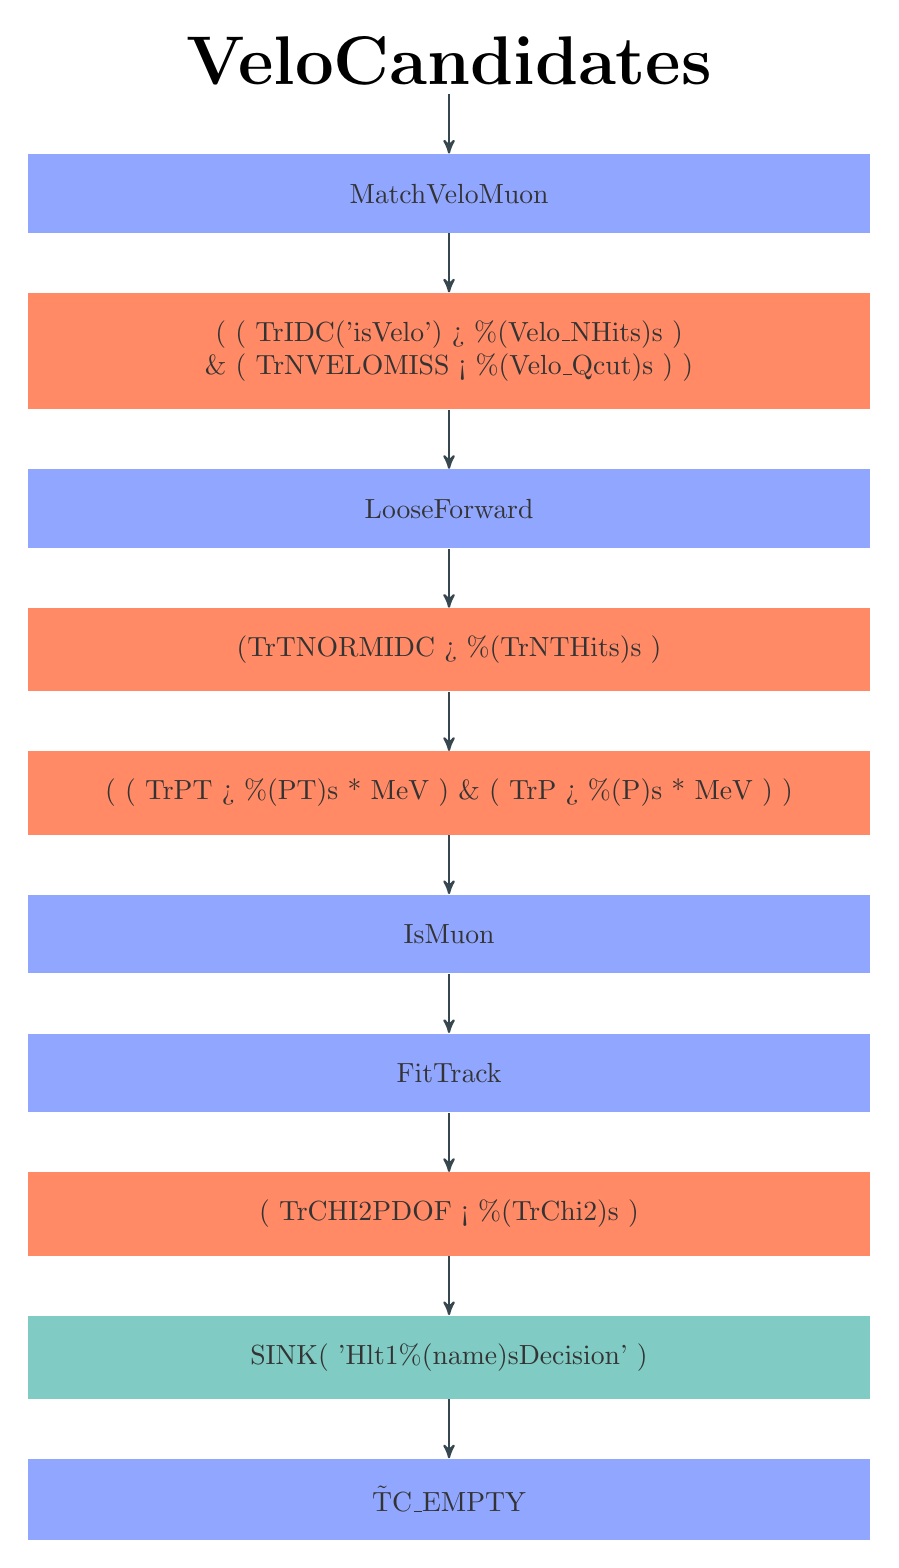
\begin{tikzpicture}[node distance=.75cm and 2.75cm]
    \node [start] (test-0) {VeloCandidates};
    \node [block, below=of test-0] (test-1) {MatchVeloMuon};
    \node [block, cut, below=of test-1] (test-2) {( ( TrIDC('isVelo') > \%(Velo\_NHits)s ) \& ( TrNVELOMISS < \%(Velo\_Qcut)s )  )};
    \node [block, below=of test-2] (test-3) {LooseForward};
    \node [block, cut, below=of test-3] (test-4) {(TrTNORMIDC > \%(TrNTHits)s )};
    \node [block, cut, below=of test-4] (test-5) {( ( TrPT > \%(PT)s * MeV ) \& ( TrP  > \%(P)s  * MeV ) )};
    \node [block, below=of test-5] (test-6) {IsMuon};
    \node [block, below=of test-6] (test-7) {FitTrack};
    \node [block, cut, below=of test-7] (test-8) {( TrCHI2PDOF < \%(TrChi2)s )};
    \node [block, sink, below=of test-8] (test-9) {SINK( 'Hlt1\%(name)sDecision' )};
    \node [block, below=of test-9] (test-10) {\~TC\_EMPTY};
    \path [line] (test-0) -- (test-1);
    \path [line] (test-1) -- (test-2);
    \path [line] (test-2) -- (test-3);
    \path [line] (test-3) -- (test-4);
    \path [line] (test-4) -- (test-5);
    \path [line] (test-5) -- (test-6);
    \path [line] (test-6) -- (test-7);
    \path [line] (test-7) -- (test-8);
    \path [line] (test-8) -- (test-9);
    \path [line] (test-9) -- (test-10);
  \end{tikzpicture}
  \caption{Flowchart of Test}
\end{figure}

\end{document}
